\subsection{Implementation}
\label{sec:implementation} 
Figure~\ref{fig:interaction} showed a high level overview of the interaction between the needed callbacks. This section will focus on an actual implementation of the given architecture. To fulfill the requirement of not being disabled or bypassed from usermode, this implemented defense is running in kernelmode and can not be accessed from usermode applications. Running applications in kernelmode is possible by using a driver and the callback functions of Figure~\ref{fig:interaction} can be used. Figure~\ref{fig:sequence} shows the actual communication between all involved objects, the \emph{Windows} kernel, the implemented driver and its callbacks and an actual process, in this case chrome.exe. The sequence diagram separates the communication into two parts represented by the colors yellow and green. The yellow part shows the interaction of the \gls{DLL} Component, the green part deals with the \gls{WPM} component. The third and last component, the process tree structure is involved in both \gls{DLL} and \gls{WPM} component. Appendix \ref{appendix:driver} shows the full code used for the implemented driver.
\newgeometry{margin=0mm,headheight=0mm,footskip=0mm,includehead,includefoot}
\pagestyle{empty}
\begin{figure*}[!p] 
 \centering
 \makebox[\textwidth]{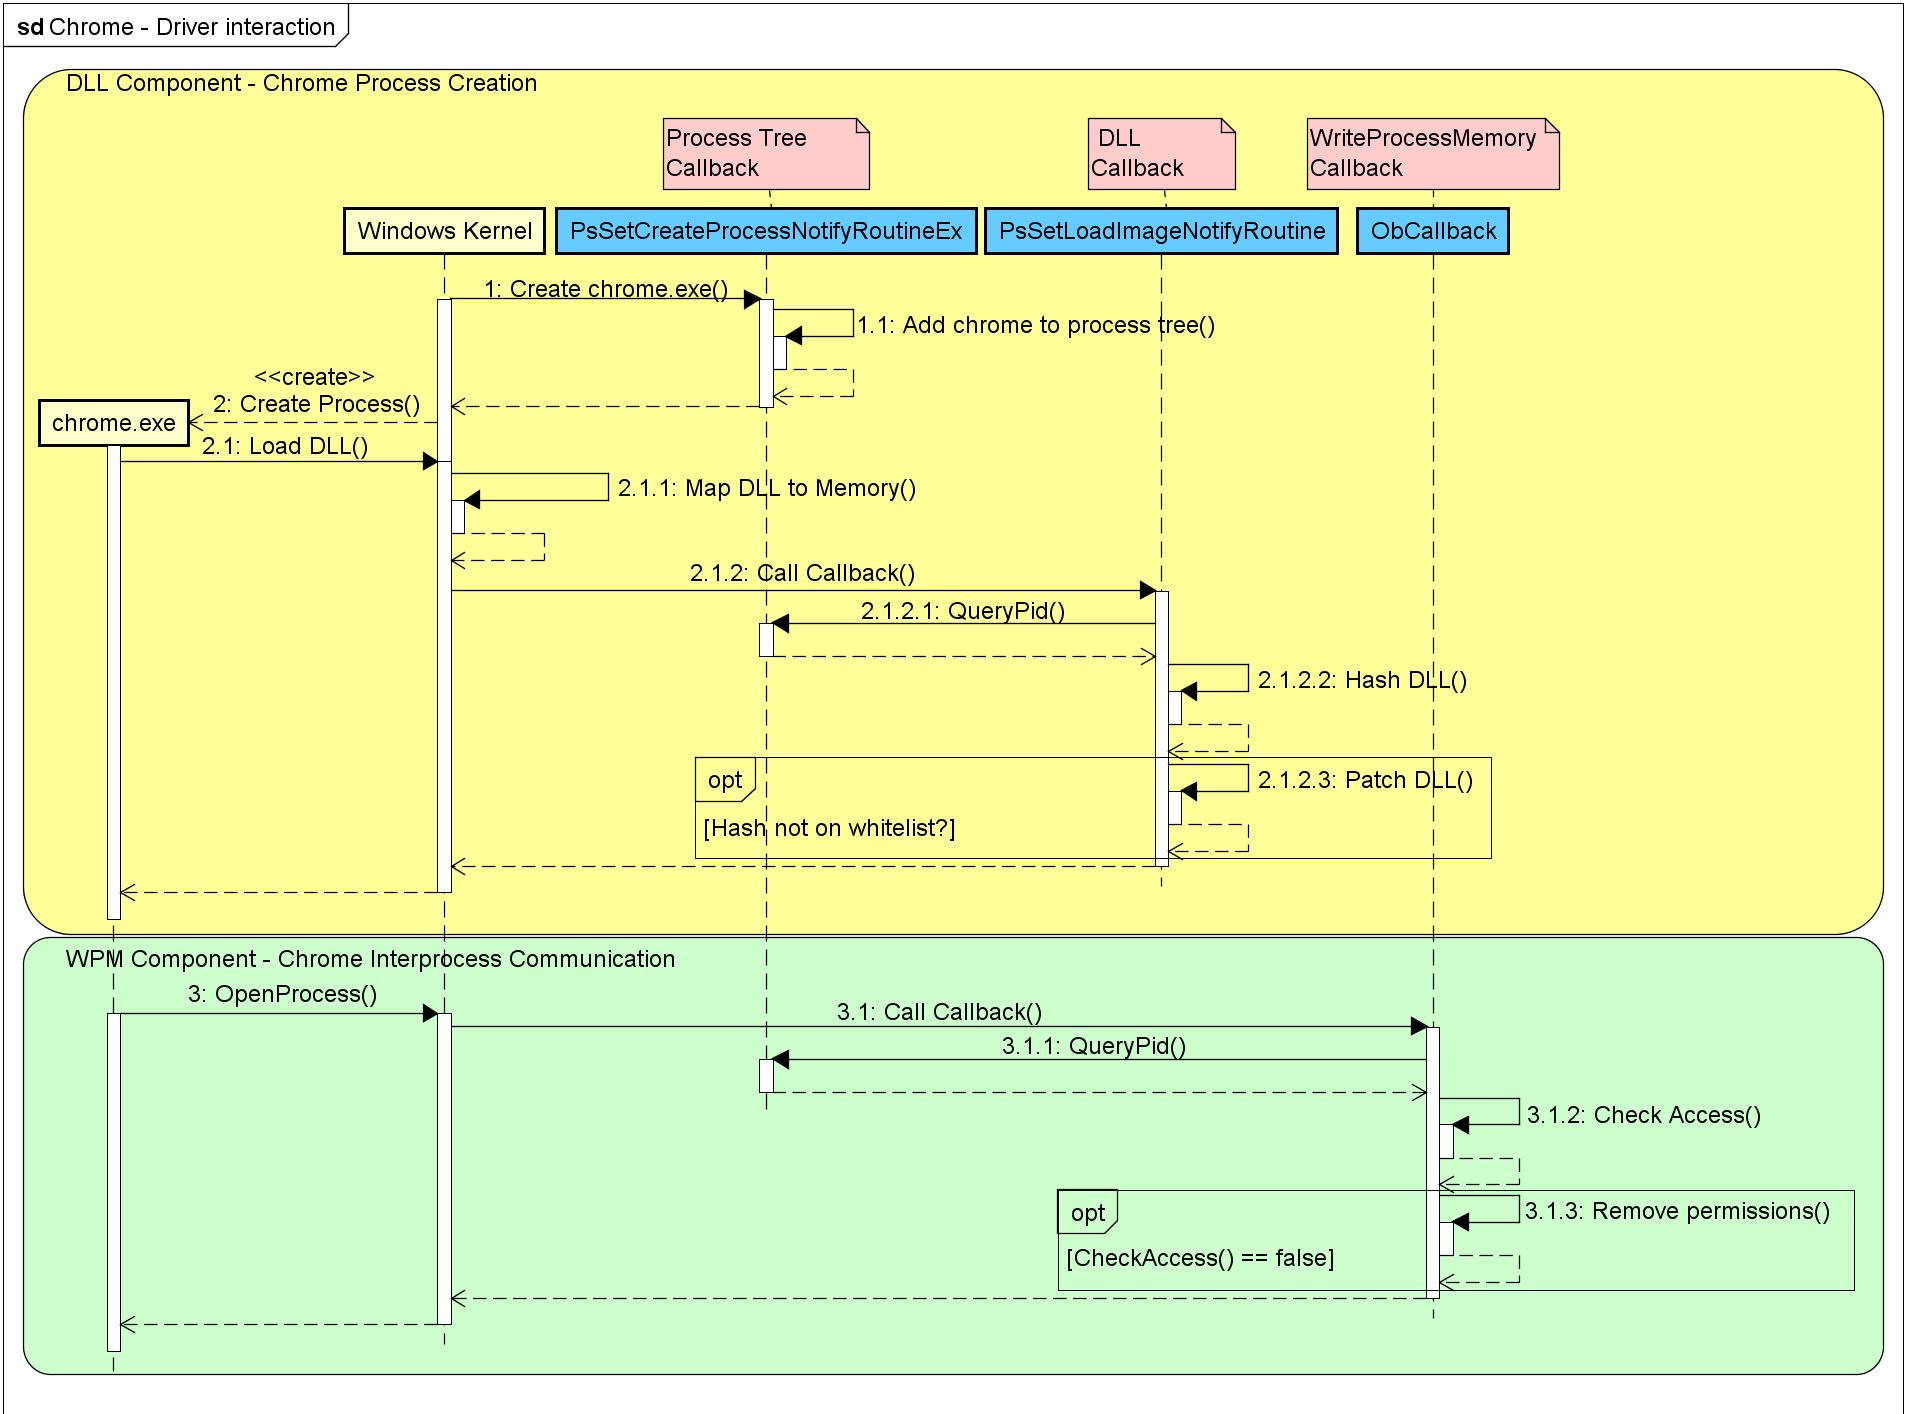
\includegraphics[angle=90,width=.85\paperwidth]{sections/implementation/driver-sequence.png}}
\caption{Sequence diagram showing the interaction between driver, \emph{Chrome} and the \emph{Windows} kernel}
\label{fig:sequence}
\end{figure*}
\restoregeometry
\pagestyle{plain}
\subsubsection{The Process Tree structure}
A naive implementation that just checks for process' executable file name may result in an access gain for the attacker. In this case the attacker could rename itself to bypass the implemented countermeasure. To prevent bypassing of the countermeasures, a process tree structure is created, which tracks the actual \glspl{PID} to keep track of process hierarchies. The process tree structure stores processes into a linked list. Figure \ref{code:code1} shows the used code to define the process tree structure. Two structs are used, the first \syscall{\_PROCESS\_LIST\_ENTRY} represents parent processes. The second, \syscall{\_PROCESS\_LIST\_ENTRY\_CHILD} represents child processes of a parent process. The linked list structure is built by calling \syscall{InitializeListHead} \cite{msdn_initlisthead}.
\begin{figure}[h]
\inputminted[breakanywhere, breaklines,fontsize=\scriptsize, frame=single, mathescape, linenos, numbersep=5pt, numbersep=5pt, xleftmargin=0pt]{c}{sections/implementation/code1.c}
\caption{Process Tree base structure}
\label{code:code1}
\end{figure}
Whenever the \emph{Windows} kernel calls \syscall{PsSetCreateProcessNotifyRoutineEx} entries are added to or removed from the linked list structure. Figure~\ref{code:code2} shows the method used for inserting such a process. At first, the process tree structure is searched for the given \gls{PID}. If the \gls{PID} is not part of the current process tree, a new entry is added. The list head for possible child processes needs to be initialized as well.
\begin{figure}[h]
\inputminted[breakanywhere, breaklines,fontsize=\scriptsize, frame=single, mathescape, linenos, numbersep=5pt, numbersep=5pt, xleftmargin=0pt]{c}{sections/implementation/code2.c}
\caption{InsertPidToTree routine of the process tree structure}
\label{code:code2}
\end{figure}
Because the process tree is used for \gls{DLL} and \gls{WPM}, a special query method is used, \syscall{FindPidInTree}. This function searches the process tree to find an existing \gls{PID} and is represented in Figure~\ref{code:code3}. At first, all parents are checked. As most processes contain only a few or no children, this is faster than iterating over all processes at once. Only if no match is found, a one level deeper search is performed. This time, children are checked. If a match is found, the corresponding parent \gls{PID} is returned, or zero otherwise. The mapping of child \glspl{PID} to parent \glspl{PID} is important to identify processes that are definitely allowed to do inter process communication.
\begin{figure}[h]
\inputminted[breakanywhere, breaklines,fontsize=\scriptsize, frame=single, mathescape, linenos, numbersep=5pt, numbersep=5pt, xleftmargin=0pt]{c}{sections/implementation/code3.c}
\caption{FindPidInTree routine of the process tree structure}
\label{code:code3}
\end{figure}

\subsubsection{The DLL Component}
The \gls{DLL} Component uses as entry point the \syscall{PsSetLoadImageNotifyRoutine} callback function. This function is executed whenever a \gls{DLL} is mapped into memory. During the function call, the process is in a suspended state and thus execution of the \gls{DLL} has not begun. However, this entry point for \gls{DLL} load prevention is not optimal, as this function call occurs after the \gls{DLL} was already mapped into memory and a pre loading callback would be better to use in this situation. Unfortunately, this callback function does not exist so far, so the implementation has to rely on the post load callback.

\medskip

To make use of \syscall{PsSetLoadImageNotifyRoutine}, the \gls{IRQL} may not be changed. Otherwise it can lead to a deadlock or even make the system crash in a blue screen of death. The \gls{IRQL} is a hardware specific flag that gets set on the processor. Depending of the chosen level, the processor may not do a context switch until the \gls{IRQL} has been changed back to a lower value. \syscall{PsSetLoadImageNotifyRoutine} operates on \gls{IRQL} \syscall{PASSIVE\_LEVEL} and special kernel mode \gls{APC} are disabled. \glspl{APC} are required to receive special event information. This can typically be found with I/O operations, where a file is being read. The kernel will fire an event as soon as the file read operation has finished, which wakes up the calling thread and execution can continue. However, reading a file without such events will always deadlock the thread. These two conditions, the \gls{IRQL} and disabled \glspl{APC} are a major limitation, because reading the \gls{DLL} file and calculating a hash is not possible inside this routine. The reason for the disabled special kernel mode \glspl{APC} is a previous call to the \syscall{KeEnterGuardedRegion} function, so a call to \syscall{KeLeaveGuardedRegion} can enable \gls{APC} events again. However, this should not be done here, as the result turns out to be unpredictable and leading to random deadlocks or failing accesses on files.

\medskip

A solution can be obtained by using a second running thread, a so called work item, which execution is handled separately by the system. The advantage of this are the enabled special kernel mode \glspl{APC} and the possibility to freely change the \gls{IRQL} during execution. One major disadvantage of this way is, that some sort of thread synchronization between the work item and the initial callback function has to be introduced. This results into driver typical busy waiting, which is still faster than non busy waiting and eventually occurring context changes. Figure~\ref{code:code4} shows code which is executed after the callback function is called. At first, it is checked if the target process is a chrome.exe process. Only in this case, further checks are done and in the other case, \gls{DLL} loading is permitted. The execution then continues with the code shown in Figure~\ref{code:code5}, which is greatly simplified. The complete function is defined in Appendix \ref{appendix:driver}. A file handle to the \gls{DLL} is obtained. Depending on the given input parameters to \syscall{PsSetLoadImageNotifyRoutine}, the given file path might be invalid. According to the \gls{MSDN} it is enough to use \syscall{ObOpenObjectByPointer} to get a file handle from a file object. As it turns out, this function is not working properly. The first call to \syscall{ObOpenObjectByPointer} succeeds and returns a valid file handle. All subsequent calls fail with \syscall{STATUS\_UNSUCCESSFUL}. Kernel debugging allows to find the reason of failure, which is an internal call to \syscall{ObpIncrementHandleCount} that returns \syscall{STATUS\_UNSUCCESFUL}. There can be found nothing with respect to this problem and it might be a bug inside the \emph{Windows} kernel itself. Therefore, manually path building is done which adds the corresponding drive letter and removes superfluous characters. Finally, after having a valid file handle, the file is read into memory and a sha256 \cite{eckert2014sicherheit} hash is generated, which is used later to compare it to a known whitelist of \gls{DLL} files.

\begin{figure}[h]
\inputminted[breakanywhere, breaklines,fontsize=\scriptsize, frame=single, mathescape, linenos, numbersep=5pt, numbersep=5pt, xleftmargin=0pt]{c}{sections/implementation/code4.c}
\caption{Code that checks if the target process is a chrome.exe process}
\label{code:code4}
\end{figure}
\begin{figure}[h]
\inputminted[breakanywhere, breaklines,fontsize=\scriptsize, frame=single, mathescape, linenos, numbersep=5pt, numbersep=5pt, xleftmargin=0pt]{c}{sections/implementation/code5.c}
\caption{The used hashing function to generate sha256 from \gls{DLL} files}
\label{code:code5}
\end{figure}
\begin{figure}[h]
\inputminted[breakanywhere, breaklines,fontsize=\scriptsize, frame=single, mathescape, linenos, numbersep=5pt, numbersep=5pt, xleftmargin=0pt]{c}{sections/implementation/code6.c}
\caption{The used patch function to destroy DLL files}
\label{code:code6}
\end{figure}
Comparing the resulting sha256 hash to a whitelist leads to two possible actions that are taken: doing nothing, in case of a match or, patching of the \gls{DLL} file, in case of no match. Figure~\ref{code:code6} shows the used patch function, that is executed whenever no match in the whitelist is found.
An initial thought could be to undo the internal \syscall{ZwMapViewOfSection}/\syscall{NtMapViewOfSection} function that loaded the \gls{DLL} into memory by calling its counter pair \syscall{ZwUnmapViewOfSection}/\syscall{NtUnmapViewOfSection} and thus removing the \gls{DLL} from memory. This will not succeed as a special lock is hold, the LdrLoadLoaderLock, that can not be accessed at this point of code. Calling the functions regardless will deadlock the driver and soon after deadlock the whole system. 

\medskip

Thus, the \gls{DLL} will only get patched, rendering it, although still residing in memory, useless. To do that, three points in memory receive modifications: the entry point address, the \syscall{DOS MZ header}, which describes the file format of a \gls{DLL} with many meta information and the entry point function. The entry point address is set to \syscall{NULL}, the entry point function will get patched with a single \syscall{ret} (0xC3) instruction to prevent execution and the memory containing the \syscall{DOS MZ header} will get zeroed. All three steps guarantee, that nothing will be able to execute from this memory mapped \gls{DLL} file and thus preventing typical \gls{DLL} injections from \syscall{SetWindowsHookEx}, the \emph{Registry} or other techniques.

\subsubsection{The WPM Component}
The \gls{WPM} component uses as entry point a callback function registered with \syscall{ObRegisterCallback}. This callback function is called whenever a process handle is created. \syscall{ObRegisterCallbacks} allows to setup a pre- and post-execution callback to modify the permissions requested. \emph{Microsoft} offers an example driver using \syscall{ObRegisterCallbacks} at \cite{github_obcallback} and shows how to modify the requested process handle permissions to prevent termination by other applications such as the task manager. In order to protect \emph{Chrome}, the same structure \emph{Microsoft} uses is used. Instead of preventing termination, the permissions of modifying a process virtual memory are removed. Figure \ref{code:code7} contains the code which is executed whenever the callback function is executed. At first, both processes, the target and the current one, need to be retrieved. Then several checks are done to see if the virtual memory modifications should be allowed. If the current and target processes have the same \gls{PID}, nothing is done. Otherwise a lookup in the Process Tree structure is done, to receive the corresponding parent \glspl{PID}. If the parent \glspl{PID} match, nothing is done. In case no match is found, the permission \syscall{PROCESS\_VM\_WRITE} is removed from the process handle and calls to \syscall{WriteProcessMemory} will fail.
\begin{figure}[h]
\inputminted[breakanywhere, breaklines,fontsize=\scriptsize, frame=single, mathescape, linenos, numbersep=5pt, numbersep=5pt, xleftmargin=0pt]{c}{sections/implementation/code7.c}
\caption{The used callback function to detect virtual memory modifications.}
\label{code:code7}
\end{figure}
